\documentclass[a4paper]{report}
\usepackage{setspace}

\pagestyle{plain}
\usepackage{amssymb}
\usepackage{graphicx}
\usepackage{color}
\usepackage{amsfonts}
\usepackage{latexsym}
\usepackage{amsmath}
\usepackage[toc,page]{appendix}
\setcounter{tocdepth}{1}
\usepackage{pdfpages}
\usepackage{todonotes}
\usepackage{hyperref}
\hypersetup{
    colorlinks,
    citecolor=black,
    filecolor=black,
    linkcolor=black,
    urlcolor=black
}

\usepackage[authoryear]{natbib}
\usepackage{algorithm}
\usepackage{algpseudocode}

% \usepackage{caption}
\usepackage{subcaption}
\usepackage{float}
\usepackage{lipsum}
\usepackage[a4paper, margin = 3cm, bottom = 2.5cm]{geometry}

\newtheorem{theorem}{THEOREM}
\newtheorem{lemma}[theorem]{LEMMA}
\newtheorem{corollary}[theorem]{COROLLARY}
\newtheorem{proposition}[theorem]{PROPOSITION}
\newtheorem{remark}[theorem]{REMARK}
\newtheorem{definition}[theorem]{DEFINITION}
\newtheorem{fact}[theorem]{FACT}

\newcommand{\nats}{\mbox{\( \mathbb N \)}}
\newcommand{\rat}{\mbox{\(\mathbb Q\)}}
\newcommand{\rats}{\mbox{\(\mathbb Q\)}}
\newcommand{\reals}{\mbox{\(\mathbb R\)}}
\newcommand{\ints}{\mbox{\(\mathbb Z\)}}

%%%%%%%%%%%%%%%%%%%%%%%%%%

% ========================================
% Title Page
% ========================================
\title{{\vspace{-14em} 
\includegraphics[scale=0.4]{Logos/ucl_logo.png}}\\
{{\vspace{2em} \Huge Beyond the Circle: Deforming Contours in Inverse Z-Transform}}\\
{\large Final Year Project Report}\\
}
\date{Submission date: \today}
\author{Roman Ryan Karim\thanks{
{\bf Disclaimer:}
This report is submitted as part requirement for the MEng degree in Mathematical Computation at UCL. It is substantially the result of my own work except where explicitly indicated in the text. The report may be freely copied and distributed provided the source is explicitly acknowledged.}
\\ \\ Dr Carolyn Phelan
\\ \\ \\ \\ Department of Computer Science
\\ University College London
\\ \\
}


% ========================================
% Report
% ========================================
\begin{document}
 
\onehalfspacing
\maketitle
\begin{abstract}

\end{abstract}

% ========================================
% Contents
% ========================================
\tableofcontents
\setcounter{page}{1}

% ========================================
% Introduction
% ========================================
\chapter{Introduction}
\section{Motivation}

\todo[inline]{High-Level overview for pricing options.}

\todo[inline]{How this problem relates to the inverse Z-transform.}

\section{Aims and Objectives}

\todo[inline]{Implementing widely used numerical methods for the inverse Z-transform.}
\todo[inline]{Testing out Levendorskii's method}
\todo[inline]{Benchmarking the performance of these methods.}

\section{Overview}

\todo[inline]{2-3 sentences of each chapter}

% ========================================
% Background
% ========================================
\chapter{Background}
"By definition, a complex number $z$ is an ordered pair ($x, y$) of real numbers $x$ and $y$, written $z = (x, y)$" \cite{kreyszig2010advanced}. In practice, complex numbers are written in the form $z = x + iy$, where $x$ and $y$ are real numbers and $i$ is the imaginary unit. The set of complex numbers is denoted by $\mathbb{C}$.


\section{$\mathcal{Z}$-Transform}
\todo[inline]{Come up with a more catchy Z-Transform title}

The $z$-transform is a transformation of a real or complex continuous time function $x(t)$, often used for discrete time signals and is commonly described as the discrete time Fourier transform (DTFT). Taking the Fourier transform of a sampled function results in

\begin{equation}
\mathcal{F}\bigg[x(t) \sum^{\infty}_{n = -\infty} \delta(t - n \triangle t)\bigg] = \int^{\infty}_{-\infty} x(t)	 \sum_{n = - \infty}^{\infty} \delta (t - n\triangle t)e^{-j\omega t} dt 
\end{equation}

\noindent We can then make use of the sifting property of the delta function.

\begin{equation}
	= \sum_{n = - \infty}^{\infty} \int^{\infty}_{-\infty} x(t) \delta (t - n\triangle t)e^{-j\omega t} dt 
\end{equation}

\begin{equation}
	= \sum^{\infty}_{n=-\infty} x(n \triangle t)e^{-j\omega nt}
\end{equation}

\noindent If we normalise the sampling interval to 1, we get

\begin{equation}
	\sum^{\infty}_{n = - \infty} x(n)e^{-j n \omega}
\end{equation}
The sequence $x(n)$ is sampled at discrete time intervals $t_n = n \triangle t$, where the sampling interval $\triangle t$ is the time between consecutive samples and the time index $n$ numbers the samples \cite{LovelessGuido2021}. 

\section{Discrete Pricing Options}

\section{Optimisation Techniques}

% ========================================
% Experiment
% ========================================
\chapter{Experiment}

\todo[inline]{Finding different parameters to use for the experiment making use of Machine Learning techniques.}

% ========================================
% Results
% ========================================
\chapter{Results}

% ========================================
% Conclusion
% ========================================
\chapter{Conclusion}
\section{Summary}

\section{Future Work}

\section{Acknowledgements}


% ========================================
% References 
% ========================================
\addcontentsline{toc}{chapter}{References}
\bibliography{references}
\bibliographystyle{apalike}

% ========================================
% Appendix
% ========================================
\begin{appendices}

\chapter{Initial Project Plan}

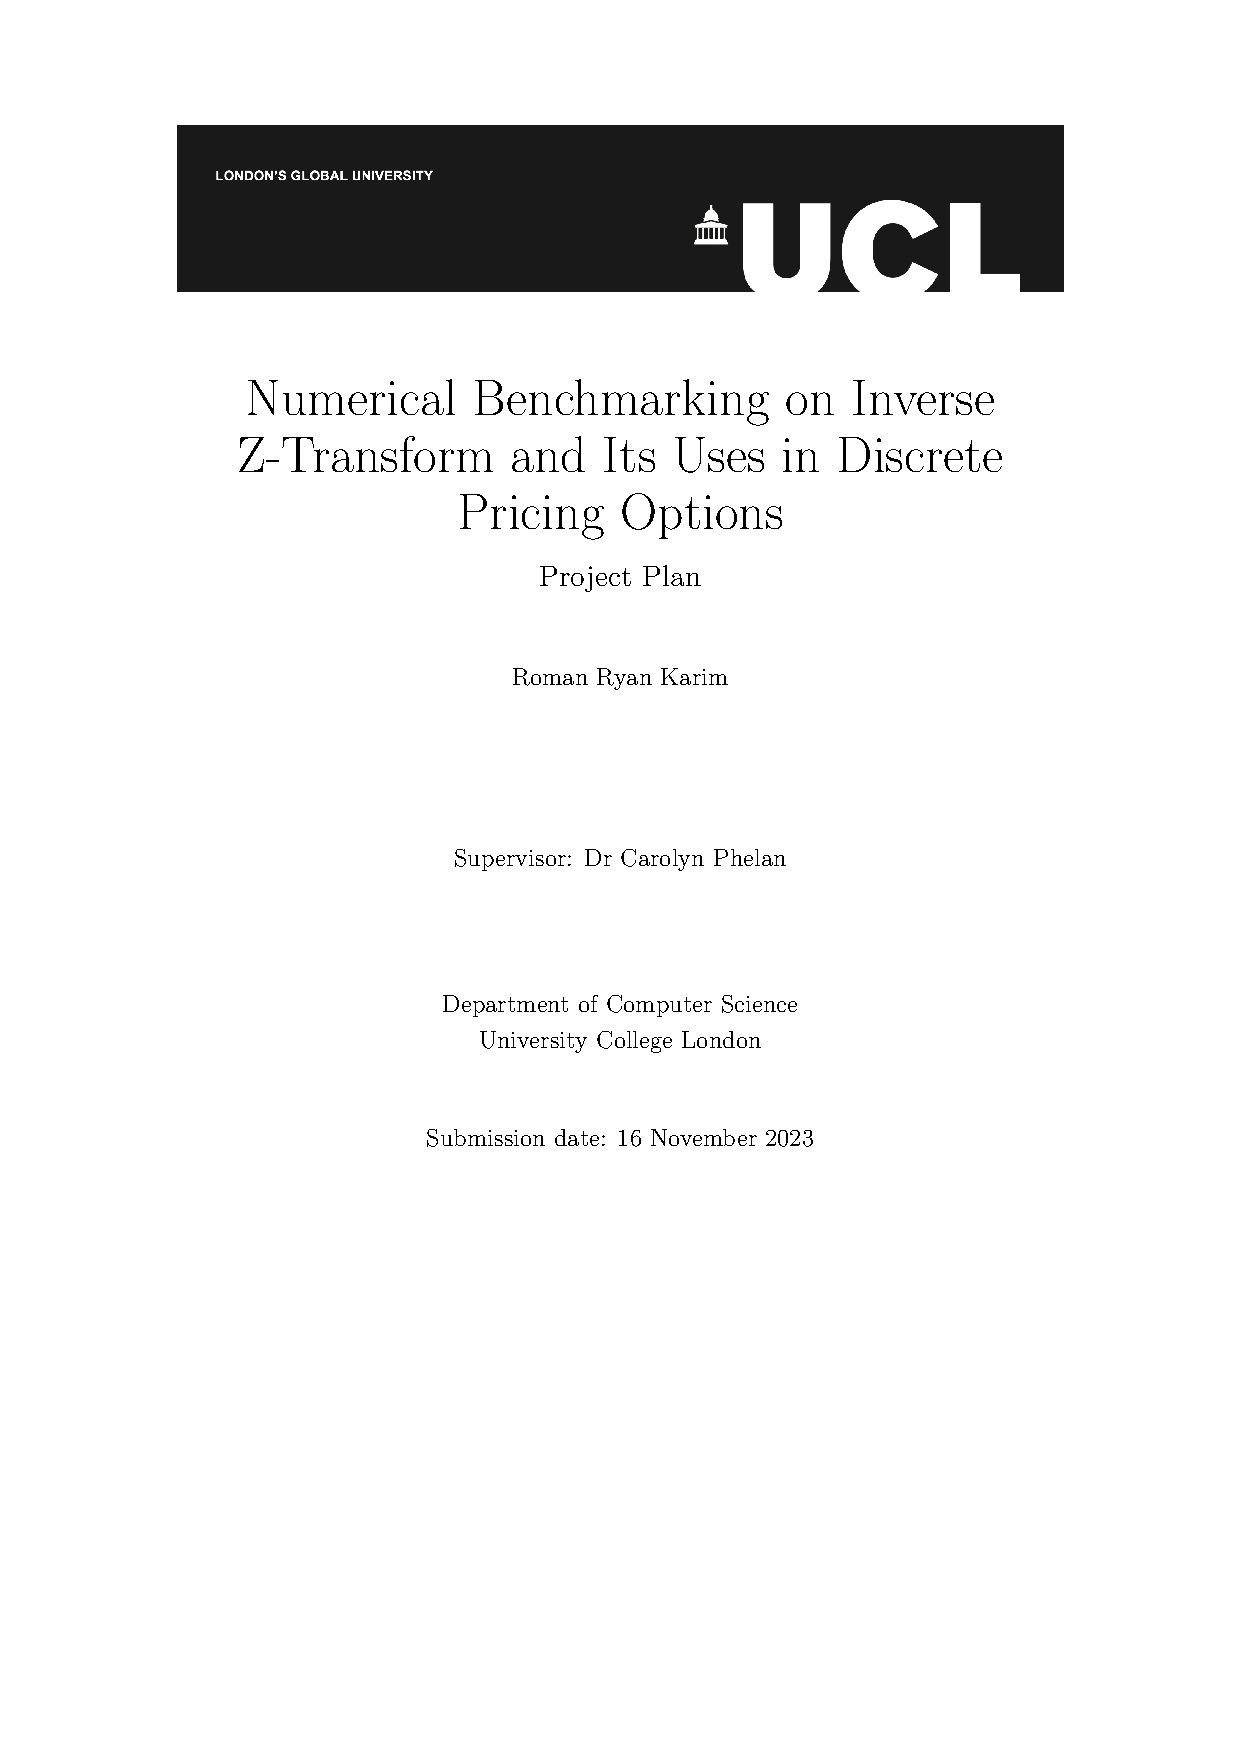
\includepdf[pages=-]{initial_project_plan.pdf}
    
\end{appendices}

\end{document}